\let\negmedspace\undefined
\let\negthickspace\undefined
\documentclass[journal]{IEEEtran}
\usepackage[a5paper, margin=10mm, onecolumn]{geometry}
%\usepackage{lmodern} % Ensure lmodern is loaded for pdflatex
\usepackage{tfrupee} % Include tfrupee package

\setlength{\headheight}{1cm} % Set the height of the header box
\setlength{\headsep}{0mm}     % Set the distance between the header box and the top of the text

\usepackage{gvv-book}
\usepackage{gvv}
\usepackage{cite}
\usepackage{amsmath,amssymb,amsfonts,amsthm}
\usepackage{algorithmic}
\usepackage{graphicx}
\usepackage{textcomp}
\usepackage{xcolor}
\usepackage{txfonts}
\usepackage{listings}
\usepackage{enumitem}
\usepackage{mathtools}
\usepackage{gensymb}
\usepackage{comment}
\usepackage[breaklinks=true]{hyperref}
\usepackage{tkz-euclide} 
\usepackage{listings}
% \usepackage{gvv}                                        
\def\inputGnumericTable{}                                 
\usepackage[latin1]{inputenc}                                
\usepackage{color}                                            
\usepackage{array}                                            
\usepackage{longtable}                                       
\usepackage{calc}                                             
\usepackage{multirow}                                         
\usepackage{hhline}                                           
\usepackage{ifthen}                                           
\usepackage{lscape}
\usepackage{multicol}
\begin{document}

\bibliographystyle{IEEEtran}
\vspace{3cm}

\title{1.2.12}
\author{EE25BTECH11012-BEERAM MADHURI}
% \maketitle
% \newpage
% \bigskip
{\let\newpage\relax\maketitle}

\renewcommand{\thefigure}{\theenumi}
\renewcommand{\thetable}{\theenumi}
\setlength{\intextsep}{10pt} % Space between text and floats


\numberwithin{equation}{enumi}
\numberwithin{figure}{enumi}
\renewcommand{\thetable}{\theenumi}


\textbf{Question}:\\
For $|x| < 1$, $\coth(x)$ can be approximated as: \hfill (EC 2007)

\begin{enumerate}
    \item[a)] $x$
    \item[b)] $x^2$
    \item[c)] $\dfrac{1}{x}$
    \item[d)] $\dfrac{1}{x^2}$
\end{enumerate}


\textbf{Solution:}\\
The hyperbolic cotangent function is defined as:

\begin{align}
    \coth(x) = \frac{\cosh(x)}{\sinh(x)}
\end{align}

To find the approximation for small x, we use the Taylor Series expansions for $\cosh(x)$ and $\sinh(x)$ centered at 0:
Expansion of cosh(x) and sinh(x)
\begin{align}
    \cosh(x): 1 + \frac{x^2}{2!} + \frac{x^4}{4!} + \dots\\
    \sinh(x): x + \frac{x^3}{3!} + \frac{x^5}{5!} + \dots
\end{align}
Now, substitute these into the $\coth(x)$ formula:
\begin{align}
    \coth(x) = \frac{1 + \frac{x^2}{2} + \dots}{x + \frac{x^3}{6} + \dots}
\end{align}
For very small values of x, we can focus on the dominant terms (the lowest power of x in the numerator and denominator):
\begin{align}
    \coth(x) \approx \frac{1}{x}
\end{align}

Correct Option: c) $\frac{1}{x}$

\begin{figure}
\centering
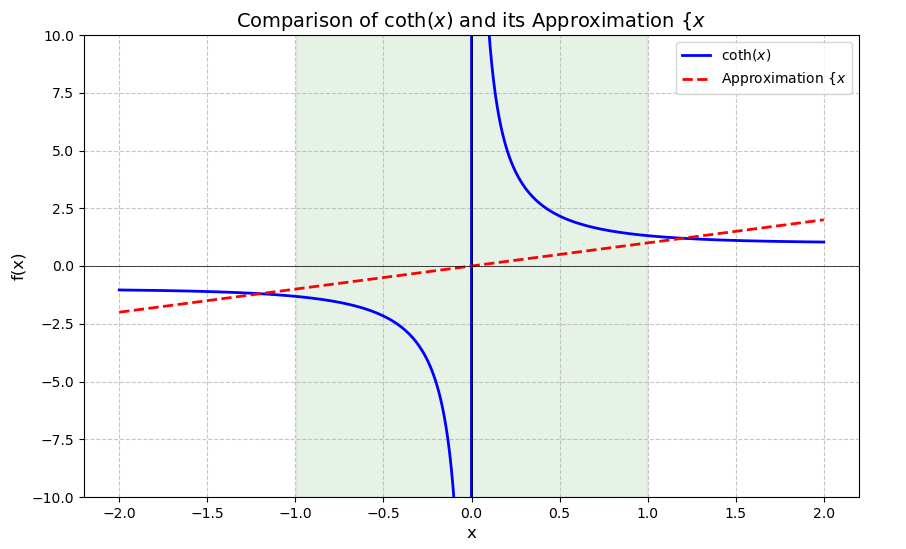
\includegraphics[width=0.75\columnwidth]{Figures/a.png}
\caption{Coth(x) and x comparision for $|x|<1$}
\label{fig:placeholder}
\end{figure}

\begin{figure}
\centering
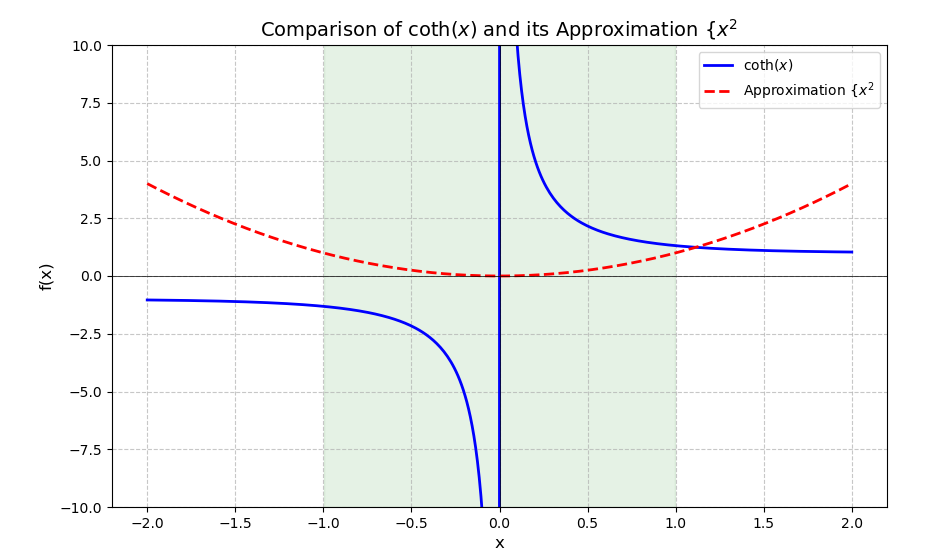
\includegraphics[width=0.75\columnwidth]{Figures/b.png}
\caption{Coth(x) and $x^2$ comparision for $|x|<1$}
\label{fig:placeholder}
\end{figure}

\begin{figure}
\centering
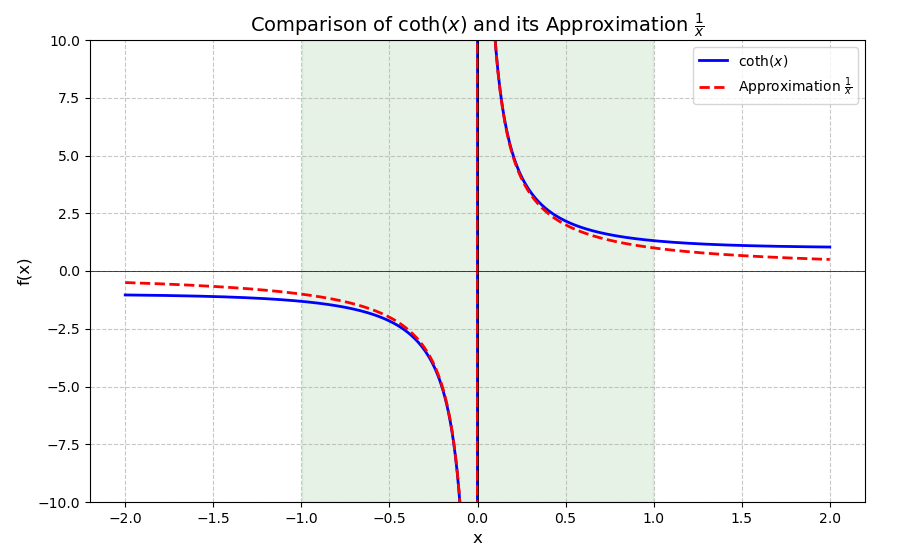
\includegraphics[width=0.75\columnwidth]{Figures/c.png}
\caption{Coth(x) and 1/x comparision for $|x|<1$}
\label{fig:placeholder}
\end{figure}
\begin{figure}
\centering
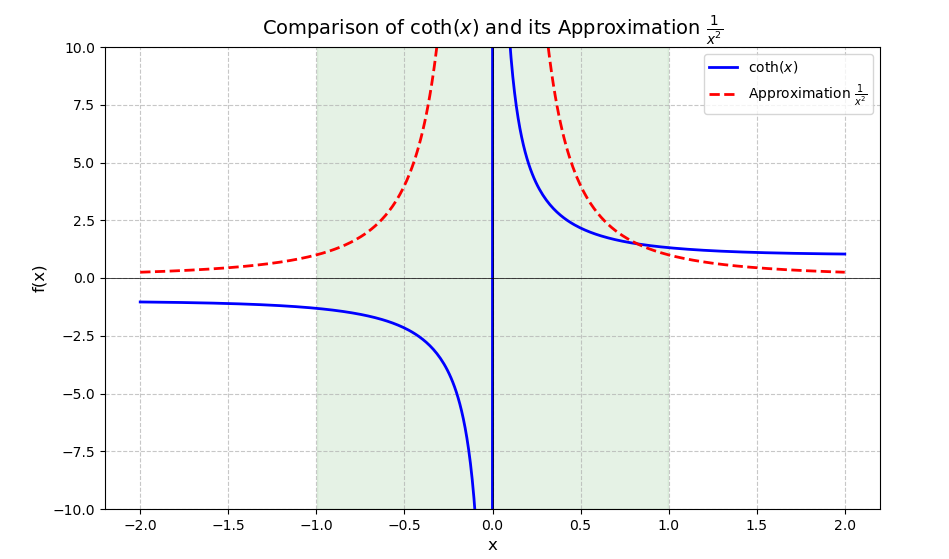
\includegraphics[width=0.75\columnwidth]{Figures/d.png}
\caption{Coth(x) and $1/x^2$ comparision for $|x|<1$}
\label{fig:placeholder}
\end{figure}
\end{document}
